\newpage

\section{Reproducing stylized facts with HMMs}
\label{Section: Stylized facts}

\textbf{Still need to figure out whether to move data section to here, deleting data section completetly or keeping it...}

\textbf{Current decoding/prediction is not really used for anything. Consider deleting or changing the analysis. Basing the section on smoothing probabilities in the rolling model might be better than showing predictions since this is what is used in forecasting in MPC framework.}

The previous section involved tuning the \jump and \mle estimators followed by an analysis showcasing how the models perform in a number of simulated environments. This section will build on the recently acquired knowledge to train the models on financial data. As such, the purpose of this section is to analyze the estimator's fit to financial returns, which is mostly analyzed by evaluating the models' ability to reproduce some well established stylized facts. As highlighted throughout section \ref{section: Data} the normal distribution provides a poor fit for financial returns and it is very difficult to train models capable of yielding the same distributional and temporal properties as those of financial returns (Cont, 2001). Researchers, including Granger \& Ding (1995b), Cont (2001) and Malmsten \& Teräsvirta (2010), have found a variety of different stylized facts that are persistent across asset returns. 

Building on the stylized facts of Granger \& Ding (1995b), Rydén et al. (1998) showed how a mixture of Gaussian distributions, theoretically can satisfy the stylized facts and subsequently attempted to fit a Gaussian HMM to S\&P 500 log returns. Rydén et al. (1998) found that most of the stylized facts could in fact be well reproduced by a Gaussian HMM, yet many of the stylized facts had to be somewhat relaxed. In particular, the researchers found the slow decay of the absolute returns to be the hardest to reproduce. This is due to the fact that HMMs by design exhibit exponential decay in their absolute autocorrelation functions. Furthermore, by splitting their data into 10 sub-samples of 1700 observations, Rydén et al. (1998) found significant changes to underlying data-generating process. Furthermore, Bulla et al. (2011) considered a similar analysis, however, they also included HMMs fitted on conditional t-distributions for which they achieved a better fit in regards to some of the stylized facts, especially those regarding higher order moments. Yet, they still found significant changes from one sub-sample period to the next, not only in their models but in the empirical data as well. As such, it can be concluded that the results from both these studies imply that the data merely fluctuates around the stylized facts of introduced by Granger \& Ding (1995b).

One inherent issue with both these authors' approach is that when dividing the empirical data into sub-samples of 1700 periods, it becomes more challenging to estimate long-memory effects from the models. Furthermore, it is also a very rough discretization of the data, which makes it more difficult to assess how the model parameters evolve across time. More recent research has tried to alleviate this with either online or rolling models such as Nystrup (2017), though he only considered the HMMs ability to reproduce squared autocorrelation functions and thus omitted analysing any of the other properties established by Granger \& Ding (1995b).

As a result, the contribution of this section to the current literature will be the estimation of rolling HMMs, through the \mle and \jump approach, as well as such models' ability to reproduce the stylized facts of Granger \& Ding (1995b). The preliminary findings indicate that the rolling models generally have a much slower decay in its absolute autocorrelation function compared to the static models of Rydén et al. (1998) and that the distributional properties are well reproduced across the data period\footnote{
With some exceptions to kurtosis in periods around Black Monday, the Financial Crisis and the COVID-19 outbreak.
}
Additionally, this is also the first study to consider how well HMMs estimated through the \jump approach reproduce the stylized facts.

The rest of the section is organized as follows. Firstly, the thesis investigate the data of which the rolling models are trained after which an overview of the rolling estimation and the model parameters is provided. Secondly, the stylized facts established by Granger and Ding (1995b) are briefly reviewed, after which these stylized facts are sought reproduced with the \mle and \jump models. When testing the models' ability to reproduce the stylized facts the distributional properties are initially estimated followed by the temporal properties. \textbf{Finally, both model's state predictions are shown together with their smoothing probabilities.}


\subsection{Data - The S\&P 500}

\textbf{Der skla noteeres at observationer som Black Monday er droppet sammen med 3 andre ekstreme observationer - se sektion 6.}

\textbf{Afsnittet bør rykkes ned til sektion 6 og forkortes. Jeg syntes figurerne over dist. og temp. properties skal i appendiks da det alligevel bliver nøgternt gennemgået i sektion 6. Alternativt skal de være en del af introen som argument for hvorfor returns er svære at modellere. Vi kan stadig beholde lidt af teksten og så henvise til figuren i appendiks.}

\textbf{Priser og returns skal merges sammen i en figur over og under hinanden. - tænker også at y-aksen på priser kan uddgøre 2/3 af højden på den figur, mens y-aksen på returns kan udgøre 1/3 af højden.}

The S\&P 500 is a stock index comprising 500 companies from the U.S. which was founded in 1957, however, the index dates back all the way to 1923 where it tracked approximately 90 stocks. The stocks that make up the index are selected by a committee which includes representation from all major segments in American industry. As such, contrary to prevailing public sentiment, the index is not simply made up of the 500 largest companies in the U.S. The S\&P 500 is a market-capitalization weighted index in which the 10 largest companies account for 27.5\% of the capitalization as per December 2020. Figure \ref{fig: SP500_index} showcases the development of the S\&P 500 index since origination as well as the log returns. 
 
\begin{figure}[H] 
    \centering
    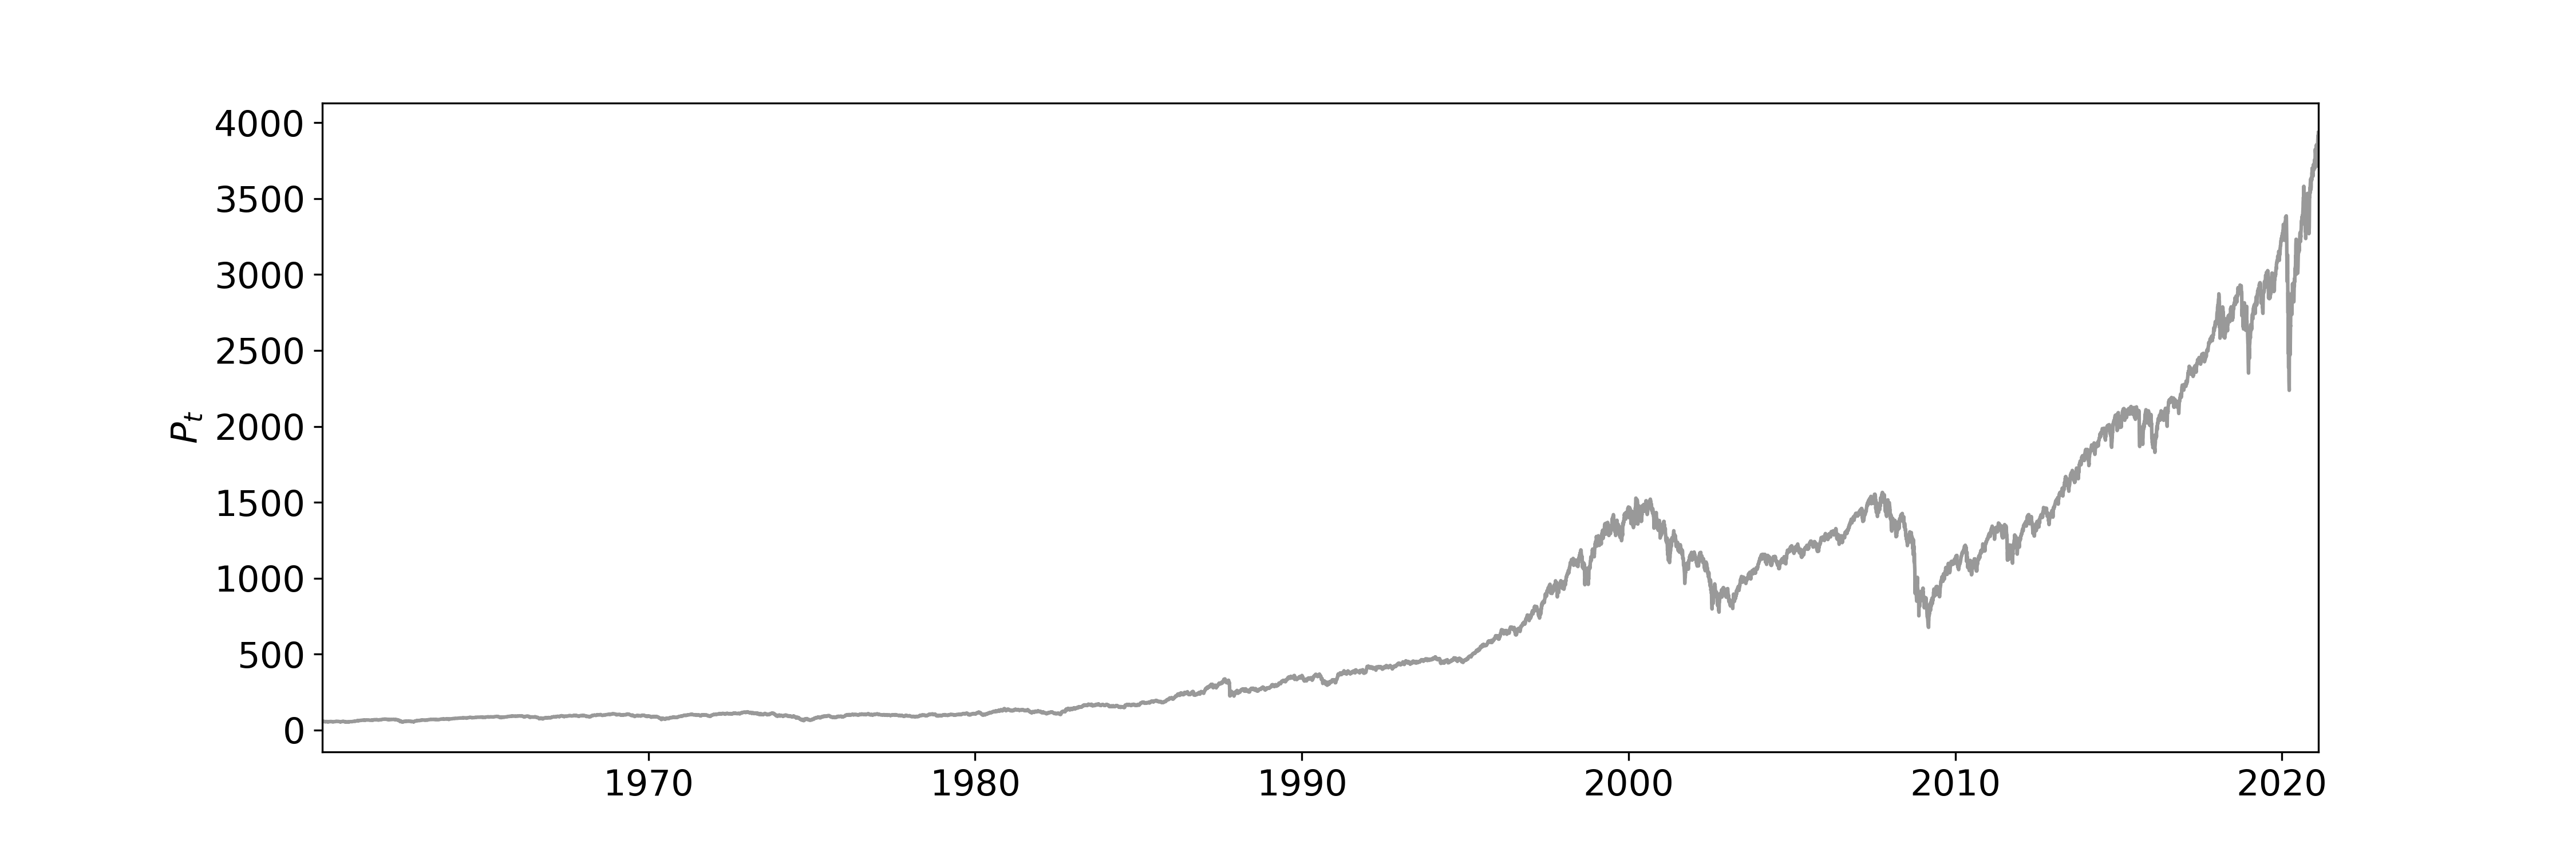
\includegraphics[width=1\textwidth]{analysis/data_description/images/SP500_index.png}
    \caption [Development of the S\&P 500] {Development of the S\&P 500 for the period 01/04/1960 to 12/02/2021.}
    \label{fig: SP500_index}
\end{figure}

The log returns are derived as $r_t = log(P_t) - log(P_{t-1})$, where $P_t$ is the adjusted closing price of the index on day $t$ and $\log$ is the natural logarithm. This is done since log returns provides a better overview of the historical market events that have caused extreme observations, for instance the Black Monday event of October 1987 which saw the S\&P 500 index drop by 22.9\% in a single day. This event is not particularly visible from the price series plot. Furthermore, it is rather impractical to try and use prices to estimate models, since stock and index prices are impossible to predict, hence a model estimation procedure should not be trained on price data.

It is evident from figure \ref{fig: SP500_index} that the 44 years of data has been impacted by the major market movements including Black Monday in October 1987 as well as the dot-com bubble of the late 90s and early 2000s. Furthermore, the attractive bull market leading up to the GFC has been well-captured by the development of the S\&P 500 Index. Lastly, the long bull market following the GFC as well as the recent COVID-19 recession appears to be well-captured by the S\&P 500 Index, thereby indicating that it is adequate for model estimation purposes. In addition, the development following the electronification of financial markets is evident since many actors, including private investors, gained access to the financial markets due to the advancement of technology in the late 90s and early 00s. This is also clearly visible from figure \ref{fig: SP500_index}


From an overall return perspective it is evident that the S\&P 500 index has been subject to a variety of turbulent market periods including the dot-com bubble and most recently the GFC and COVID-19 recession. Interestingly, the S\&P 500 index only recovered from the dot-com bubble a few months prior to the financial crisis of 2008. In the period following the financial crisis the S\&P 500 has been performing increasingly well resulting in an upward trajectory until the recent COVID-19 correction, after which the index reached the present all time high. The fact that the S\&P 500 index has captured the most recent and dramatic market turmoil throughout the last 60 years, further establish that it captures the varying nature of economic regimes. Furthermore, another neat property of the S\&P 500 is the fact that it dates back to 1957, hence there is a large amount of data that can be used to train the subsequent HMMs. For comparison, popular European indices like the DAX 30 originated in 1999, thus shortening the available data considerably.

Additionally, another the choice of relying on the S\&P 500 index for estimation purposes is based on the fact that it is a one of the leading American indices by market capitalization. Secondly, contrary to for instance the Nasdaq Composite Index, the S\&P 500 is not exclusively focusing on a specific sector like information technology, hence it should capture the economics trends across sectors accordingly. As such, the thesis treats it as a baseline index in terms of uncovering economic-regimes. The main critique of using the S\&P 500 index is that it exclusively entails American companies, however, from a macroeconomic perspective the U.S. economy serves as a fundamental leading indicator of how the remaining world economy is progressing, hence it is valid to argue that US stocks will be the first to be impacted by changing economic regime. Taking into consideration the aspect of early regime detection, this means that the fact that the index is composed purely of American companies serves as a strength. Furthermore, North American companies makes up almost 2/3 of alternative indices like the MSCI World, hence no matter which large popular index that will be used, there is bound to be a heavy skew and over-representation towards American stocks.


\begin{figure}[H] 
    \centering
    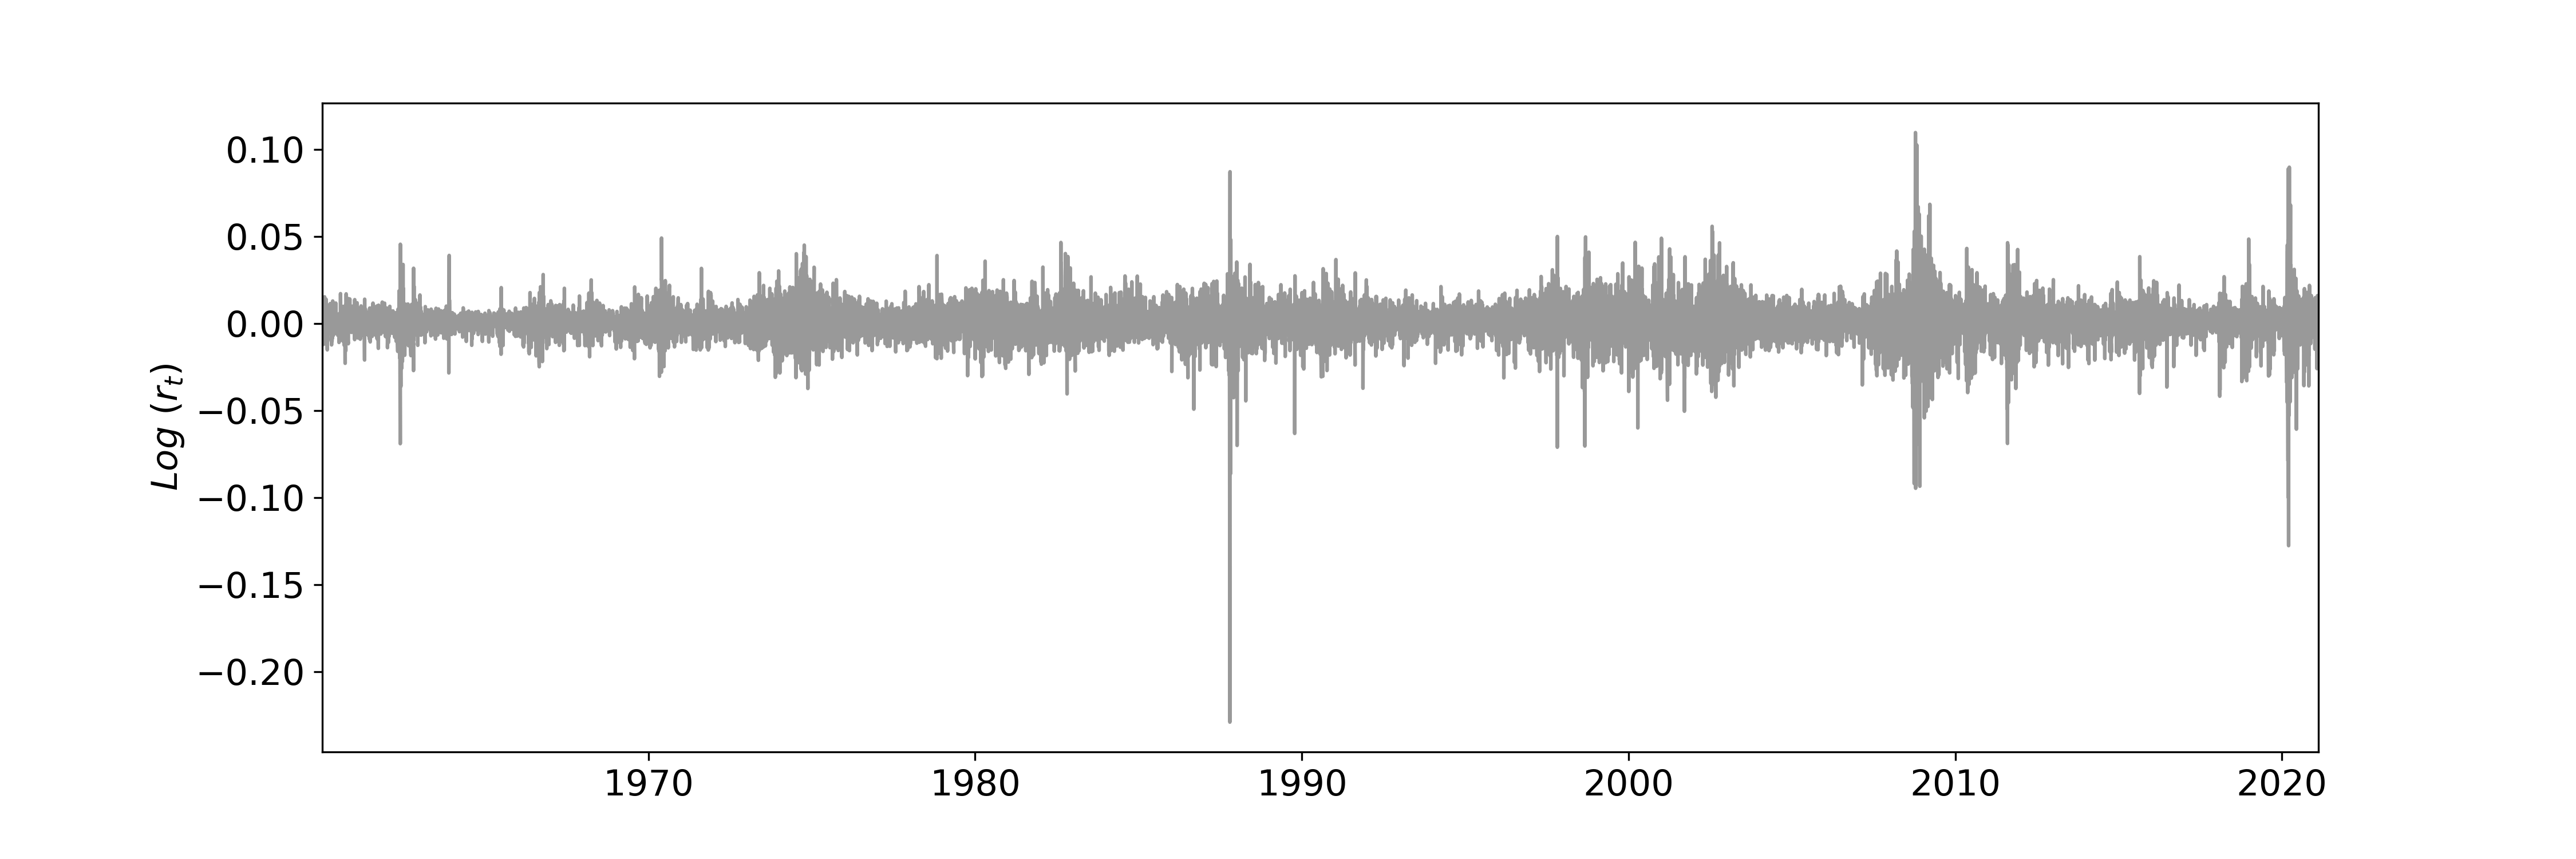
\includegraphics[width=1\textwidth]{analysis/data_description/images/SP500_log_returns.png}
    \caption [Plot of the log returns for the S\&P500 index across time] {Plot of the log returns for the S\&P500 index across time. \textbf{Figur skal være en del af priser. Ret y-akse}}
    \label{fig: log_returns_all_indices}
\end{figure}

In order to capture the summary statistics of the daily S\&P 500 log returns, as well as the annual Sharpe ratio and JB statistic, table \ref{tab:summary_stats_S&P500} has been constructed below. As such, it is apparent that the distribution is left skewed and strongly leptokurtic, however, this is not a surprising finding given the studies conducted by Granger \& Ding (1995b) as well as Cont (2001), in which identical stylized facts of financial returns were uncovered and explored substantially. The critical value for the Jarque–Bera test statistic at a 99.9\% significance level is 14.13, hence table \ref{tab:summary_stats_S&P500} clearly highlights that the Jarque–Bera test strongly rejects the hypothesis that the log returns of the S\&P 500 follow a Gaussian distribution.

\begin{table}[H]
\small
\caption{Summary statistics for the annualized S\&P 500 log returns.}
\centering
\begin{tabular}{c c c c c c c c c c} 
\hline\hline
Observations & Mean & STD & Skewness & Excess Kurtosis & Min & Max & Annual Sharpe & JB-stat \\
\hline
15,385 & 0.0709 & 0.1631 & -1.0353 & 23.8338 & -0.2290 & 0.1096 & 0.4350 & 27,926 \\
\hline
\end{tabular}
\label{tab:summary_stats_S&P500}
\end{table}
 

\subsection{Rolling estimation}
\label{Sec: rolling estimation}

The analysis now turns to estimating the \mle and \jump models on the S\&P 500 log returns covering the period 1960-2020. It should be noted that four very extreme observations\footnote{The observations include Black Monday, two trading days during the financial crisis and one observation during the outbreak of Covid-19.}
have been replaced with $\pm$ 6 times the standard deviation of the data. An important result from the simulation study was that the models became more stable with larger sample sizes in which the parameters generally appeared to stabilize between samples of 1000 and 2000 observations. As already mentioned, the window length is essentially a hyper-parameter that can be tuned and the exact choice boils down to a trade-off relationship between bias and variance. A shorter rolling window will, all else equal, result in a faster adaption to changes in the underlying economic regimes but the estimate will be more noisy as fewer observations are used when deriving the model parameters. This might result in the model adapting to "wrong" signals, which might affect the underlying trading strategy by decreasing risk-adjusted returns. A rolling window of 1700 days will be considered in this analysis as the model parameters should generally be stable at this length and this also makes it appropriate to draw direct comparisons to previous studies including Rydén et al. (1998), Bulla et. al (2011) and Nystrup (2017).

The estimation procedure for the rolling model is as follows. For each time step $t$ an HMM is estimated by the \mle and \jump procedures using the previous 1700 daily log returns. Once trained, the rolling window moves one time period forward to $t+1$ and repeats the procedure. The results of the rolling estimation for the \mle and \jump models based on a 2-state Gaussian HMM are shown in figure \ref{fig: MLE estimation rolling parameters} and \ref{fig: Jump estimation rolling parameters} respectively.

\begin{figure}[H] 
    \centering
    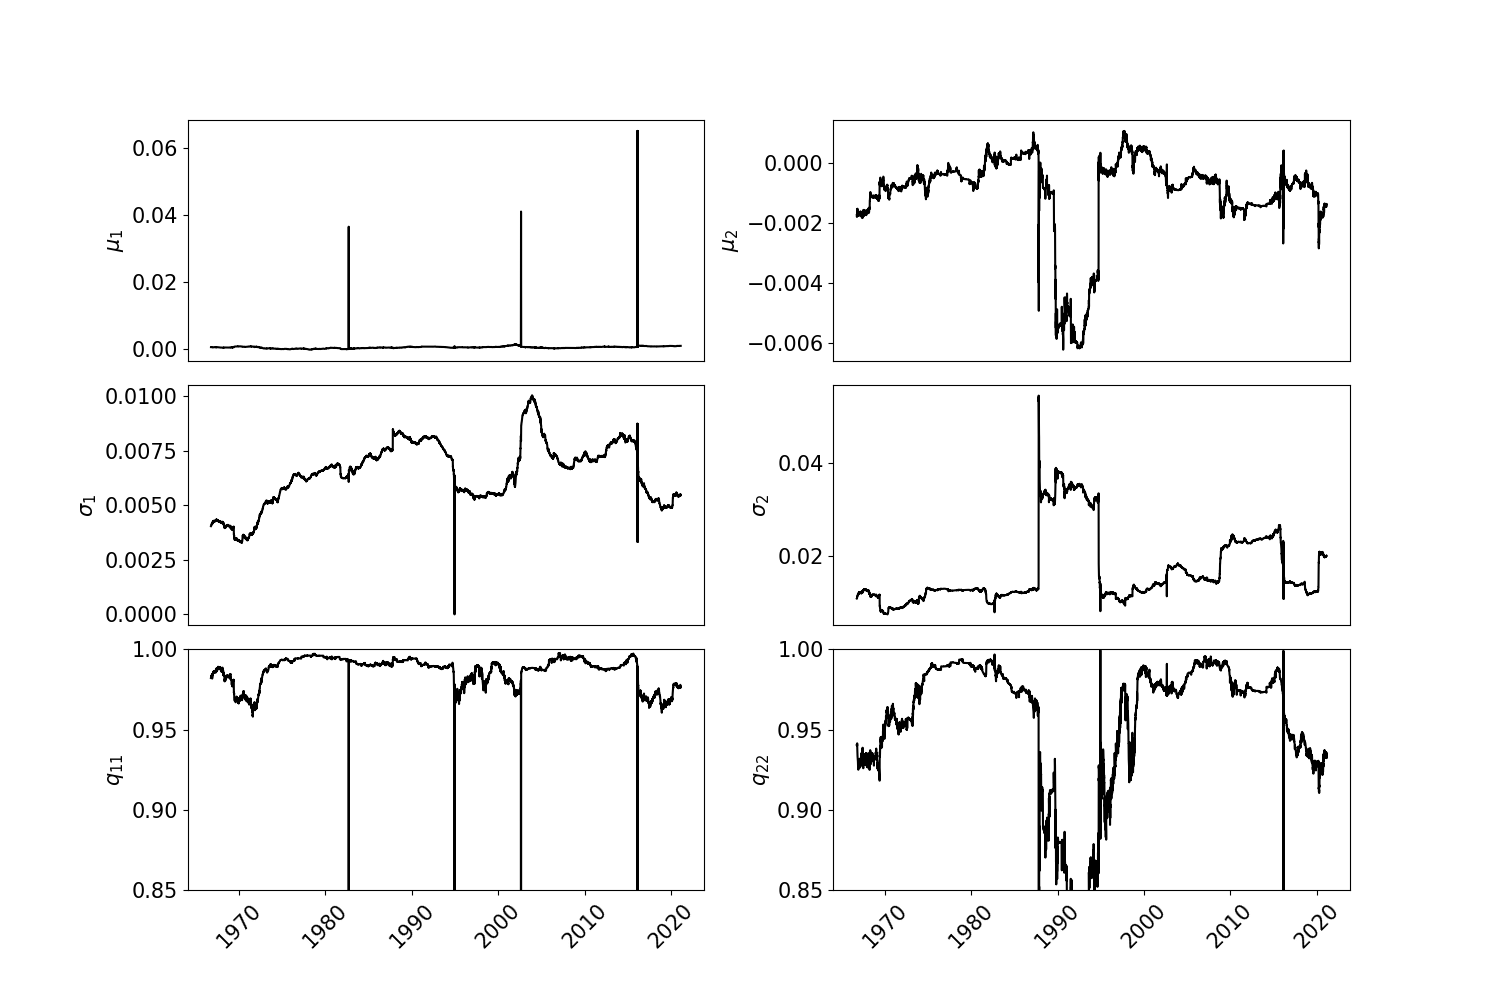
\includegraphics[width=1.0\textwidth, height=0.5\textheight]{analysis/stylized_facts/images/2-state MLE HMM rolling params.png}
    \caption[Rolling estimation based on the \mle estimator]{Rolling estimation based on the \mle estimator. The parameters are derived from a 2-state Gaussian HMM using a rolling window of 1700 days.}
    \label{fig: MLE estimation rolling parameters} 
\end{figure}

\begin{figure}[H] 
    \centering
    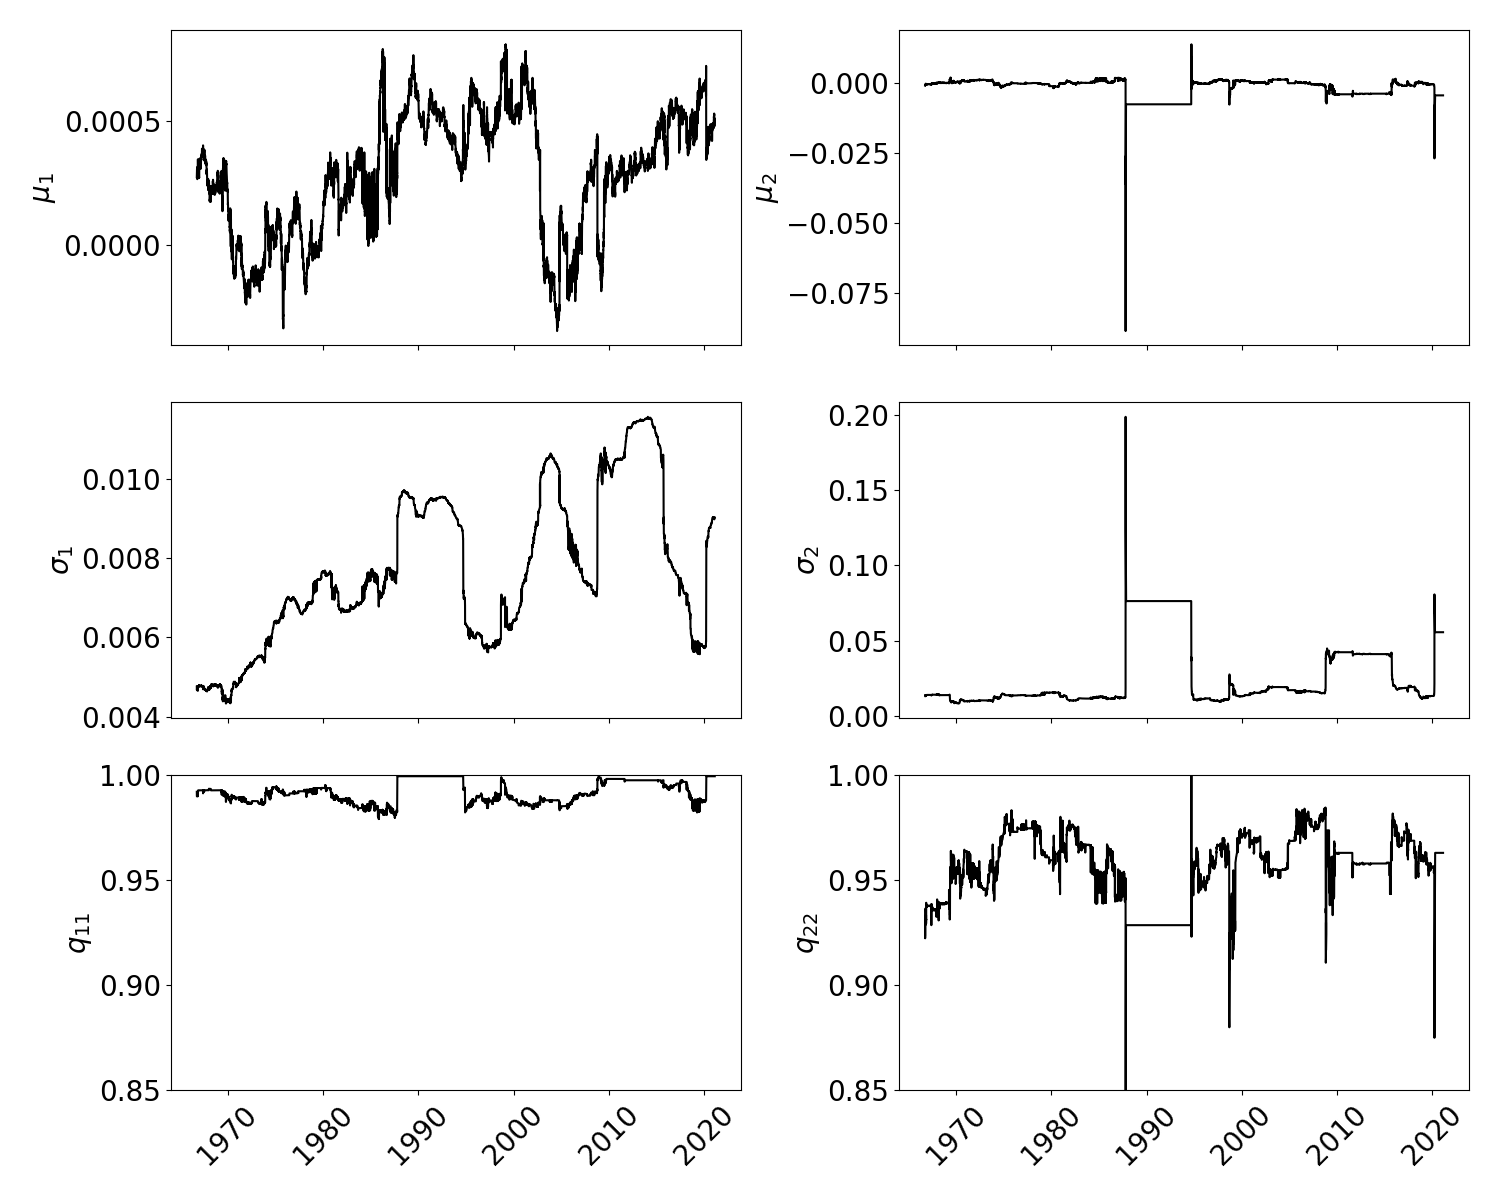
\includegraphics[width=1.0\textwidth, height=0.5\textheight]{analysis/stylized_facts/images/2-state JUMP HMM rolling params.png}
    \caption[Rolling estimation based on the \jump estimator]{Rolling estimation based on the \jump estimator. The parameters are derived from a 2-state Gaussian HMM using a rolling window of 1700 days.}
    \label{fig: Jump estimation rolling parameters} 
\end{figure}

From figure \ref{fig: MLE estimation rolling parameters} and \ref{fig: Jump estimation rolling parameters} it is evident that neither the mean nor variance parameters exhibit stationarity across time regardless of whether the estimation procedure relies on \mle or \jump approach. Starting with the \mle approach, shown in figure \ref{fig: MLE estimation rolling parameters}, the rolling window length of 1700 observations is particularly visible in the high-variance state during recessions. This is especially evident during Black Monday in 1987 and during the financial crisis in 2008 in which $\sigma_2$ spikes only to return to its old level roughly 1700 trading days later. This is an interesting behaviour because the most extreme observations from Black Monday and the financial crisis have been replaced with $\pm$ 6 times the standard deviation of the data. Yet, during these periods many other extreme returns take place and it is those observations that are responsible for the general change in $\sigma_2$. In addition, it is even more interesting that both periods of increased variance in $\sigma_2$ lies at roughly the same level. This could imply that the high-variance state fluctuates around some long term level in which large deviations only occur for extreme events such as the financial crisis and the COVID-19 recession. It could also imply the need for a third 'outlier' state with a low unconditional probability to handle these periods, but as shown by Bulla et al. (2011) such a model is often inferior to a two-state model hence it does not lead to smaller variations in the model parameters.

Interestingly, figure \ref{fig: MLE estimation rolling parameters} reveals that the mean for the first state is largely time-varying, and it has a notably large increase during the financial crisis. The same holds true for the mean in the high-variance state, especially during periods of economic turbulence, although this parameters decreases rather than increases during these dramatic periods. This development can be explained by the fact that economic history prescribe that it is highly unlikely that a large market crash is followed by an additional large market crash shortly after. As such, the model provides a good estimation for the mean in both states. When analysing the non-constant transition probabilities resulting from the \mle approach in figure \ref{fig: MLE estimation rolling parameters} it can easily be inferred that the sojourn times are mostly persistent in the low-variance state. Contrary, the transition probabilities $q_{22}$ of the high-variance state are characterised by a higher degree of fluctuations across time, mostly evident during the period following Black Monday. This means that the HMM will predict much shorter sojourn times in the high-variance state. This is a natural consequence of the properties of the transition probabilities because when $q_{22}$ decreases $q_{21}$ increases as $q_{22} + q_{21} = 1$, hence a low value of $q_{22}$ will result in more frequent transitions between states.

Moving on to figure \ref{fig: Jump estimation rolling parameters} it is evident that the \jump procedure also captures the time-varying nature of the underlying HMM parameters. The results are quite similar to those of the \mle estimator, however, the $\mu_1$ is now practically zero and the fluctuations of $\mu_2$ in the high-variance state are more abrupt during periods such as Black Monday and the financial crisis when compared to the \mle estimator. Yet, it is also evident that the high-variance state in general seem more stable with the \jump estimator in periods outside of economic turbulence. In addition, the rolling windows are also evident from the \jump approach since $\sigma_2$ spikes during Black Monday after which the parameter stabilizes at a new level, only to fall down to its original level approximately 1700 days after the event. Curiously, when analysing $\sigma_2$ the level reached during Black Monday and the financial crisis is no longer roughly equal thus rejecting the idea of two long-run levels in $\sigma_2$ when the models are estimated through the \jump framework. 

The biggest improvement of running the \jump framework as opposed to the \mle approach is seen through the estimation of the transitions probabilities for both states. Just as in the simulation study, when comparing $q_{11}$ and $q_{22}$ in figure \ref{fig: MLE estimation rolling parameters} to figure \ref{fig: Jump estimation rolling parameters} it appears that the transitions probabilities are much more stable across states when estimating the model parameters using the \jump approach. Furthermore, it appears that both model estimation procedures suggest a similar level for some of the parameters. For instance, $\sigma_1$ generally fluctuates around a level of 0.005 to 0.010 for both approaches. This provides a high degree of confidence since it is unlikely that two different estimation procedures should arrive at similar parameters randomly. Conclusively, by analysing figure \ref{fig: MLE estimation rolling parameters} and \ref{fig: Jump estimation rolling parameters} it appears that the \jump approach provides persistent transition probabilities across time, thereby suggesting that its the strongest methodology, however, further analysis of the reproduction of the stylized facts has to be conducted before this can be cemented.

Finally, figure \ref{fig:stylized_facts_rolling_moments} shows the estimated unconditional first four moments of $r_t$ as well as for the \jump and \mle estimators. As such, it is evident that both the \mle and \jump model are able to reproduce the first two moments quite well, since the mean and variance matches that of $r_t$ across all time periods.

\begin{figure}[H] 
    \centering
    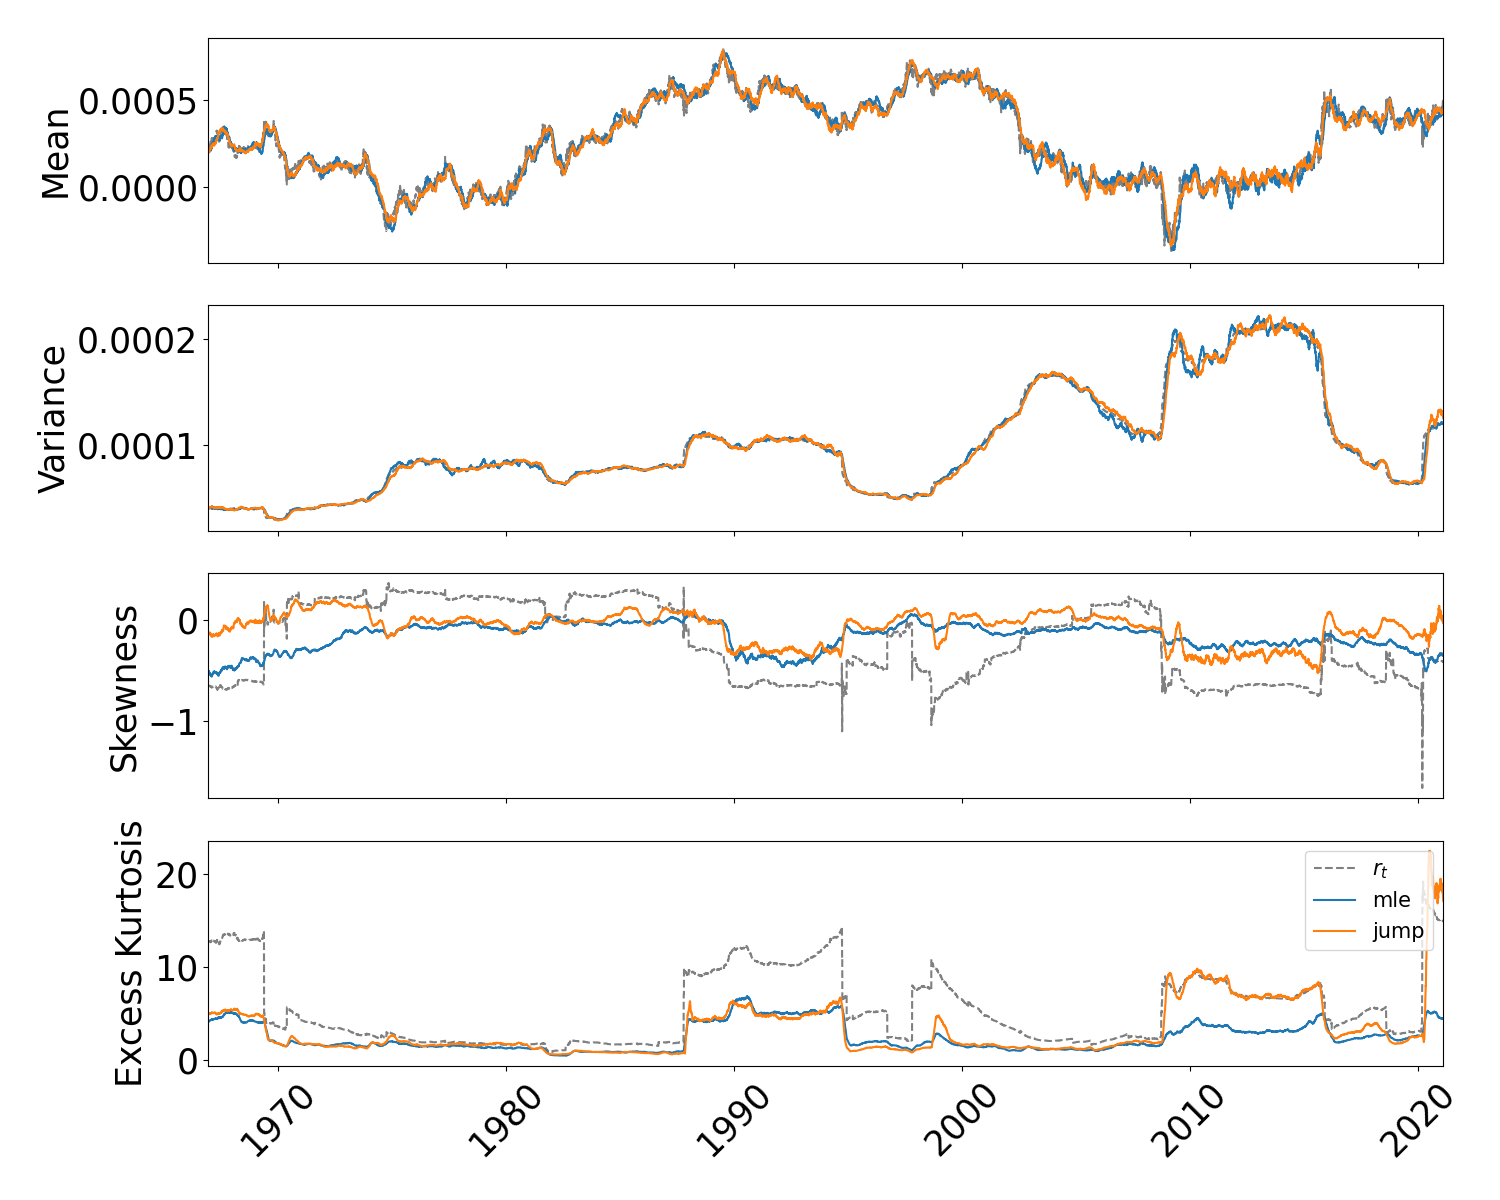
\includegraphics[width=1.0\textwidth, height = 0.4\textheight]{analysis/stylized_facts/images/moments_regular.png}
    \caption[Development of the first four moments from the estimated models and $r_t$]{Development of first four moments from the estimated models compared to $r_t$ using a rolling window of 1700 days. Model estimates are calculated using Monte-Carlo simulations.}
    \label{fig:stylized_facts_rolling_moments} 
\end{figure}

Unsurprisingly, the estimates of skewness and kurtosis are more error-prone especially during periods of economic turmoil such as during Black Monday. Still, the results are quite similar to those obtained by Bulla (2011) except that this analysis shows the full evolution of parameters over the period. When further analysing the skewness it is clear that the model parameters fluctuate around that of the data and are predominantly negative during the entire period across both models. This suggest that more observations fall into the left part of the distribution. The same conclusion is apparent for the excess kurtosis where the estimates of both models fluctuate around those of the log returns. Curiously, Bulla (2011) tended to 'overshoot' kurtosis in many of his 10 sub-samples when using t-distributions whilst blaming HMMs using Gaussian distributions for not being able to capture higher levels of kurtosis. It is then interesting to observe that apart from Black Monday, the \jump estimator is fitting kurtosis particularly well especially during the financial crisis. Additionally, the time-varying nature of the first four moments in figure \ref{fig:stylized_facts_rolling_moments} further cements the appropriateness in using rolling estimations as a static model would not have been able to capture this non-stationary data generating process.

\subsection{Reproducing the stylized facts of Granger \& Ding (1995b)}
\label{section:stylized_facts_GD}

As the parameters of the rolling models have been estimated and shown, the analysis now turns to defining the stylized facts established by Granger \& Ding (1995b) before attempting to reproduce them to uncover whether the utilized models obtain a better fit compared to Rydén et al. (1998) and Bulla (2011). The temporal and distributional properties, established by Granger \& Ding (1995b) are as follows.

\textbf{Tekst efter TPx skal indentes \newline}
TP1: Returns $r_t$ are not autocorrelated (except for, possibly, at lag 1). \newline
TP2: $|r_t|$ and $r_t^2$ are the 'long memory' i.e. their autocorrelation functions decay slowly starting from the first order autocorrelation and $corr(|r_t|, |r_{t-k}|) > corr(r_t^2, r^2_{t-k})$. The autocorrelations remain positive for many lags and the decay is much slower than the exponential rate of a typical ARMA model. \newline
TP3: The Taylor effect $corr(|r_t|, |r_{t-k}|) > corr(|r_t|^{\theta}, |r_{t-k}|^{\theta})$, $\theta \neq 1$. Autocorrelations of powers of absolute returns are highest at power one. \newline
TP4: The autocorrelations of $sign(r_t)$ are negligibly small.

The three distributional properties are as follows.

\textbf{Tekst efter DPx skal indentes \newline}
DP1: $|r_t|$ and $sign(r_t)$ are independent\newline
DP2: $|r_t|$ has the same mean and standard deviation \newline
DP3: The marginal distribution of $|r_t|$ is exponential (after outlier correction)

In addition, it should be noted that an exponentially distributed variable (DP3) $x_t$ has the following properties.

PED1: $E(x_t) = \sqrt{Var(x_t)}$ (Same as DP2) \newline
PED2: $E[x_t-E(x_t)]^3 / (Var(x_t))^{\frac{3}{2}} = 2.$ \newline
PED3: $E(x_t-E(x_t))^4 / (Var(x_t))^{2} -3 = 6.$

In the analysis conducted by Rýden et al. (1998) and Bulla et al. (2011) it has been proven that DP1 holds as a natural consequence of the construction of HMMs and that TP1 \& TP4 is not violated in practice. Since DP1, TP1 and TP4 have previously been very well reproduced the expectation is that the models presented in this thesis are able to avoid deviating too much from these stylized facts. As previously mentioned, the more difficult stylized facts to reproduce, include DP2, DP3, TP2 and TP3. Interestingly, both Ryden et al (1998) and Bulla (2011) had difficulty in reproducing these. As such, it will be the analysis of these stylized facts that are central in the coming sections starting out with the distributional properties.

\subsection{Distributional properties}
\label{Sec: Distributional properties}

In this section the analysis will focus on reproducing the distributional properties DP2 and DP3, as shown in figure \ref{fig:stylized_facts_moments_bulla_abs}, which presents the mean-standard deviation ratio, skewness and excess kurtosis of $|r_t|$ and the fitted models.

\textbf{Consider shrinking the y-axis for kurtosis.}
\begin{figure}[H] 
    \centering
    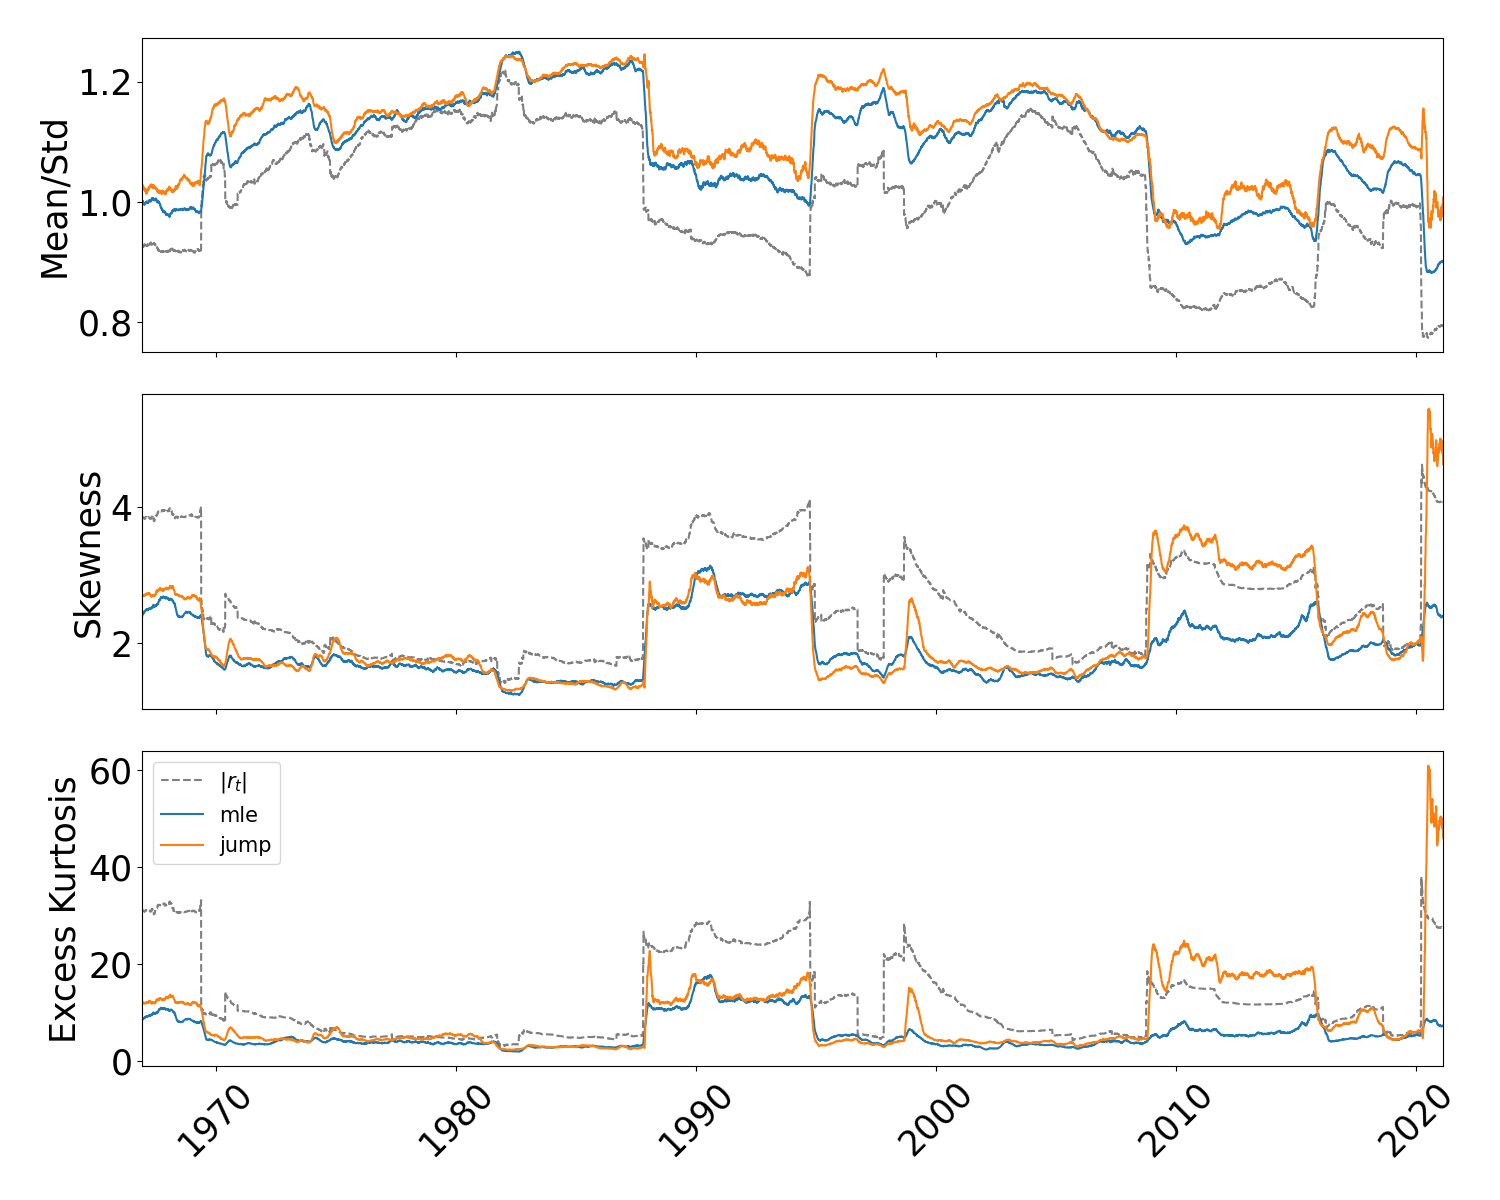
\includegraphics[width=1 \textwidth, height=0.4\textheight]{analysis/stylized_facts/images/moments_bulla_abs.png}
    \caption[$|r_t|$ and the models' distributional properties]{$|r_t|$ and the models' distributional properties. The top panel shows the mean to std ratio, the middle panel shows the skewness and the bottom panel shows the excess kurtosis.}
    \label{fig:stylized_facts_moments_bulla_abs} 
\end{figure}

When analysing the ratio of the mean and standard deviation (DP2/PED1), it can be seen that the mean is higher than the standard deviation for the predominant part of the period. This holds for both models as well as $|r_t|$ although the log returns experience a larger decline in the ratio during periods of economic turbulence. Therefore, it appears that neither of the two models sway too far away from 1, thereby indicating that the mean of the absolute returns is approximately equal to the standard deviation of the absolute returns for both models. Both the \mle and \jump models seem to fluctuate in the interval [1.0 : 1.25], which is in accordance with the findings by Rydén et al. (1998) who noted that PED1 has to be somewhat relaxed, meaning that the mean is allowed to be slightly larger than the standard deviation.

\textbf{We need a better explanation for why the models might underestimate skewness in most of the period.}

Having analysed whether the models satisfy PED1 and DP2 the final distributional property to consider is PED2 and PED3 in DP3. This is due to the fact that in order for DP3 to be satisfied the models must exhibit the properties of PED1, PED2 as well as PED3 simultaneously. Since it was just shown that DP2 holds for both models, and PED1 and DP2 are identical in their construction, it can be concluded that PED1 holds for both models. Moving on to PED2 it is evident that both the \mle and \jump model underestimate skewness in most of the period, however, it appears that the \jump model achieves a much better fit of skewness in the period following the financial crisis of 2008. Interestingly, it is clear from figure \ref{fig:stylized_facts_moments_bulla_abs} that the \mle model better matches the skewness property of PED2 (i.e. that it equals 2) compared to not only the \jump model but also the data $|r_t|$ itself. It should be noted though, that the original DP3, and thus PED2, by Granger \& Ding (1995b) only hold for outlier corrected data, for which the property generally seem to hold for both models and log returns as shown in figure \ref{fig:stylized_facts_moments_bulla_abs_outliers}. This will be analyzed further in the end of this section. 

Furthermore, it is evident that both models seem to underestimate the skewness of the empirical data $|r_t|$ particularly during the period following Black Monday as well as the extraordinary bull-market leading up to the dot-com bubble. As such, the finding is a testament to the on-going issue in which even advanced models are unable to capture the full extent of the fat tails in distributions of financial returns. This finding is further backed by the fact that it appears that both models are able to reproduce the skewness in non-volatile market periods, however, the errors arrive when the rolling model contains observations from turbulent market periods. Despite this, it appears that both models are able to capture the changing skewness and excess kurtosis around the time of large market movements. This is evident throughout the figure, but particularly around the time of the GFC. The fact that both models are able to do so is particularly promising as it provides substantial evidence towards the adequacy of the models. The fit of the models could be further improved by increasing the number of states, however, the problem with such an option is that it significantly increases the risk of overfitting (Bulla 2011). As such, it can be concluded that both models somewhat reproduce PED2.

The final property that the models must satisfy in order for DP3 to be met is PED3. As such, the models must be able to exhibit and match an excess kurtosis of 6. It is clear from figure \ref{fig:stylized_facts_moments_bulla_abs} that the \mle model slightly underestimates the excess kurtosis for the predominant period of time, however, similar to the observations of the skewness, the model approximately matches an excess kurtosis of 6 in most of the period, since its average over the period is 5.51. The \jump model, however, fluctuates around the kurtosis of $|r_t|$ with it being smaller during the period following Black Monday, slightly larger during GFC and much larger during the Covid-19 outbreak. This is in line with the \jump model's slightly larger fluctuation in its parameter estimates of $\mu_2$ and $\sigma_2$ during these periods compared to the \mle model. This is quite a satisfactory results as both Rydén et al. (1998) and Bulla (2011) underestimated kurtosis of Gaussian HMMs throughout their studied time periods.

To summarize the findings above it is clear that both the \mle and the \jump models are able to somewhat reproduce the properties of PED1 to PED3, hence it can be concluded that DP3 approximately holds. This is similar to the conclusion reached by both Rydén et al (1998) and Bulla (2011), although they only tested HMMs estimated through the \mle methodology. As such, this section contributes to the quantitative finance literature by showcasing that the stylized facts introduced by Granger \& Ding (1995b) can in fact also be somewhat reproduced by a \jump model. As such, the thesis has extended on the introduction of \jump estimation procedure for HMMs by Bemporad el at. (2018) by proving that it matches the properties of the stylized facts associated with returns on financial assets.

\subsubsection{Outlier-corrected data}

As a final remark on the distributional properties, outlier corrected data limited to the boundary of the closed interval $[\bar r_t - 4\hat\sigma, \bar r_t + 4\hat\sigma]$ will be subject to analysis. As noted by Granger \& Ding (1995b), DP3 was found to only hold on outlier corrected data and even though the above findings were somewhat satisfactory, the analysis is repeated for outlier corrected data. The results are shown in figure \ref{fig:stylized_facts_moments_bulla_abs_outliers}. It can be concluded from the figure that the results are similar to those of Bulla (2011), since he did not find large changes between the full data and the outlier corrected data in regards to whether the models reproduce the distributional properties. The mean to standard deviation ratio has risen in magnitude, but the shapes remain largely unchanged. The same conclusion holds for skewness and kurtosis. As a result, the major difference is simply that results have shifted towards the values of an exponential distribution (PED1-3), but the shapes of the curvatures remain rather unchanged.

\textbf{Begge modeller er her meget tættere på $|r_t|$ end for ikke outlier-corrected data. Men det er kun fordi momenterne har taget et lodret skift ned. Spørgsmålet er om outlier-corrected data vil give bedre density forecasts i den efterfølgende porteføljeøvelse?}

\begin{figure}[H] 
    \centering
    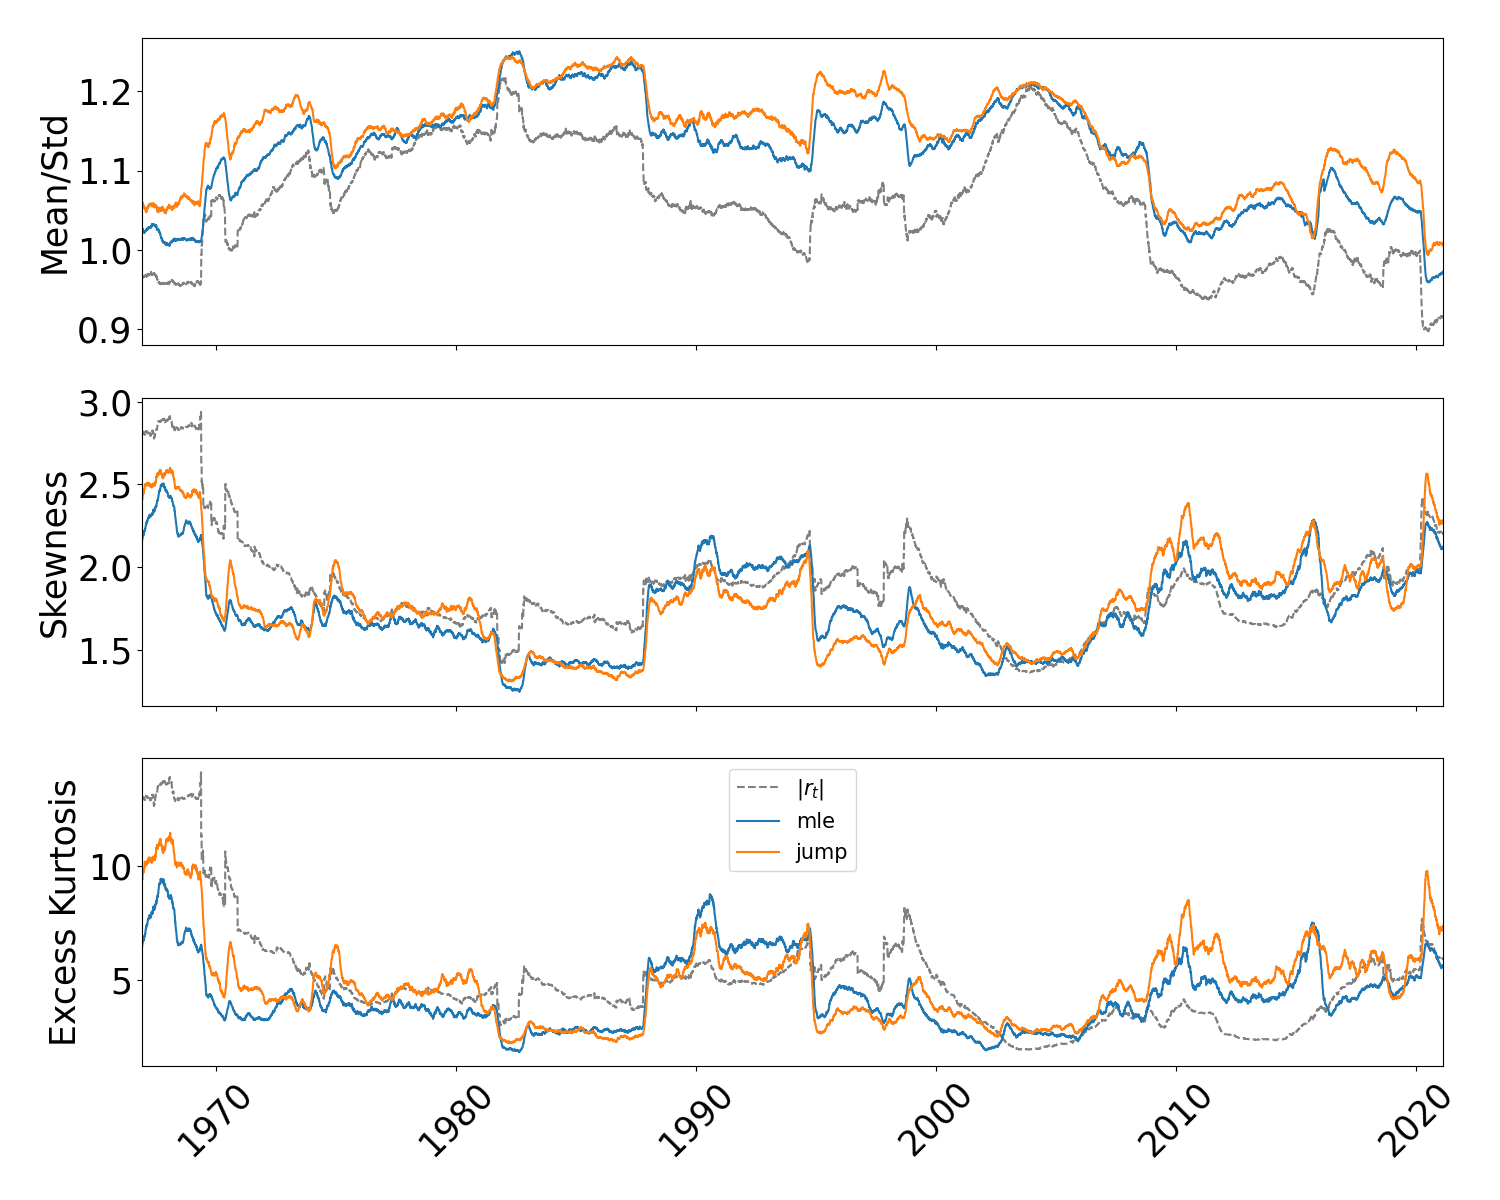
\includegraphics[width=1.0\textwidth, height = 0.4\textheight]{analysis/stylized_facts/images/moments_bulla_abs_outlier.png}
    \caption[$|r_t|$ and the models' outlier corrected distributional properties]{$|r_t|$ and the models' outlier corrected distributional properties. The top panel shows the mean to std ratio, the middle panel shows the skewness and the bottom panel shows the excess kurtosis. \textbf{Consider moving to appendix}}
    \label{fig:stylized_facts_moments_bulla_abs_outliers} 
\end{figure}

\subsection{Temporal properties}
\label{Sec: Temporal properties}

Having analyzed the distributional properties, the next logical step is to check the temporal properties as defined by Granger \& Ding (1995b). As mentioned earlier, previous research suggest that HMMs are able to reproduce most of the stylized facts quite well, however, Rydén et al. (1998) and Bulla (2011) found that HMMs are inadequate when it comes to reproducing the slow decay of the autocorrelation function of absolute daily returns which is often referred to as volatility clustering. Rydén et al (1998) considered this the most difficult stylized fact to reproduce for HMMs.

As such, most of this section will be dedicated to reproducing TP2, however, TP3 will also be covered. TP1 and TP4 are shown in appendix \ref{appendix:sign_rt}. The section is structured as follows. Initially, the authors provide some initial thoughts into why both Rydén et al. (1998) and Bulla (2011) might have had difficulty in reproducing the slow decay in the absolute autocorrelation function. The analysis then proceeds to show how the rolling models have a much slower decay in their absolute autocorrelation functions when compared to the models of Rydén et al. (1998) and Bulla (2011). Secondly, TP3 is sought reproduced by the \mle and \jump models and finally the analysis will briefly show that TP1 and TP4 are not violated.

\subsubsection{Preliminary thoughts on the ACF in static versus rolling models}

This section provides some insights into the differences for the autocorrelation function when it is derived from the full sample compared to several sub-samples. This is used to further motivate the use of rolling models. Figure \ref{fig:stylized_facts_acf_data} shows the autocorrelation of $|r_t|$ on the full sample as well as the average autocorrelation of sub-samples each containing 1700 observations. It is evident from the figure that the decay is more exponential for the sub-samples and by lag 200 the absolute autocorrelation is practically insignificant wheres the absolute autocorrelation for the full sample remains significant until lag 430, thereby exhibiting a slower decay. The faster decay in the sub-samples is most likely a result of the periods without excess risk and economic turmoil. These periods cause very low estimates of the ACF, as the volatility clustering is less significant in these periods, thereby increasing the speed of the decay. In any case, it is clear that the 'long-memory' effect has decreased in the bottom panel of figure \ref{fig:stylized_facts_acf_data}.

\begin{figure}[H] 
    \centering
    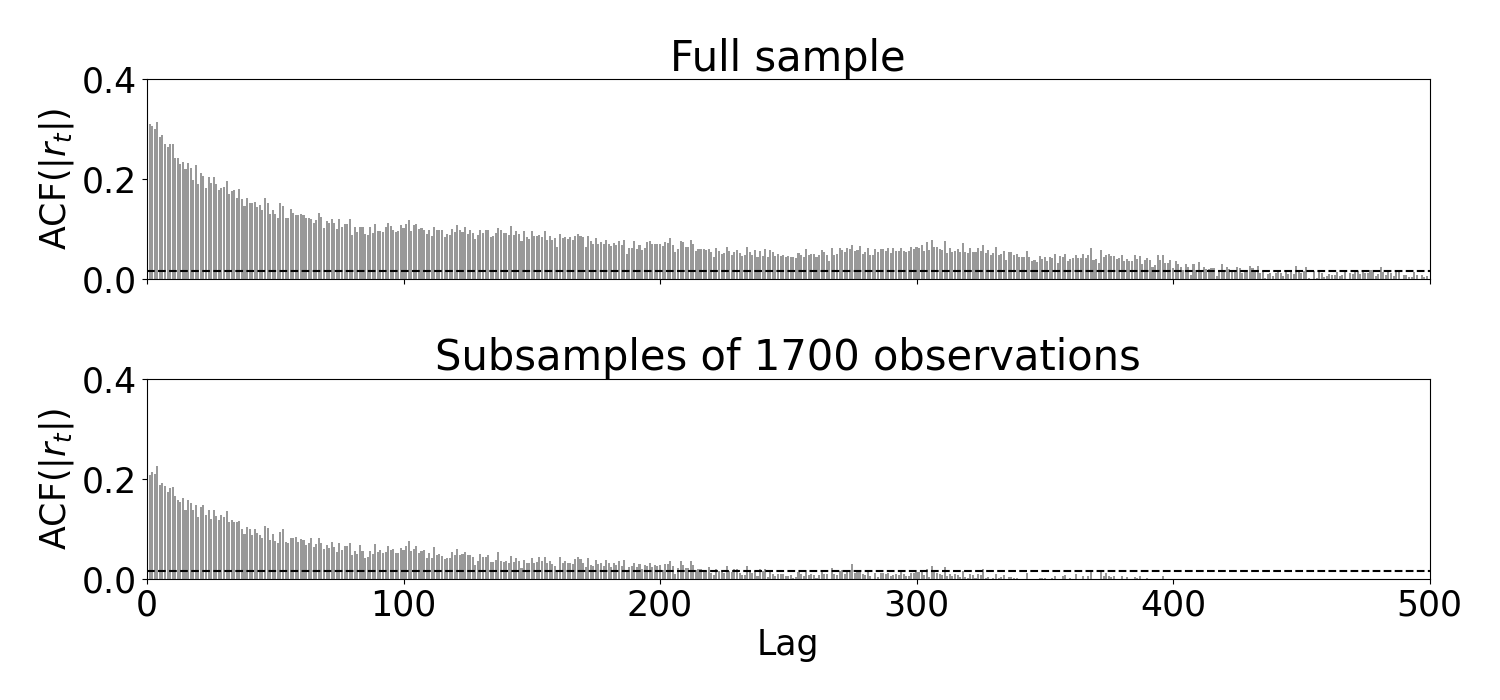
\includegraphics[width=1.0\textwidth]{analysis/stylized_facts/images/acf_data.png}
    \caption[Autocorrelation function of $|r_t|$ on full sample and subsamples]{Autocorrelation function of $|r_t|$. The top panel shows the ACF estimated on the full sample and the bottom panel shows the average ACF when the data is split into rolling subperiods of 1700 observations.}
    \label{fig:stylized_facts_acf_data} 
\end{figure}

This finding should already make one suspicious of estimating static models in a few sub-periods as Rydén et al. (1998) and Bulla (2011) did. To show the performance of the models in such a setup the procedure by Rydén et al. (1998) and Bulla (2011) is repeated. The results are shown in figure \ref{fig:stylized_facts_acf_plots_sub_periods}. As already mentioned, it is evident that there exists clear differences in the level of ACF between the sub-periods, with some periods exhibiting quite high levels of autocorrelation and other periods in which it dies down within 50 lags. The performance of both the \mle and \jump model is roughly as reported by Bulla (2011), in which the decay is generally much faster for the models than for the log returns. One interesting finding is that the \mle model appears to fit the empirical autocorrelation quite well in sub-period 3 and 8, which are periods of turmoil. Having shown how the models would have performed in a static scenario, the same analysis will now be conducted for the rolling model.

\begin{figure}[H] 
    \centering
    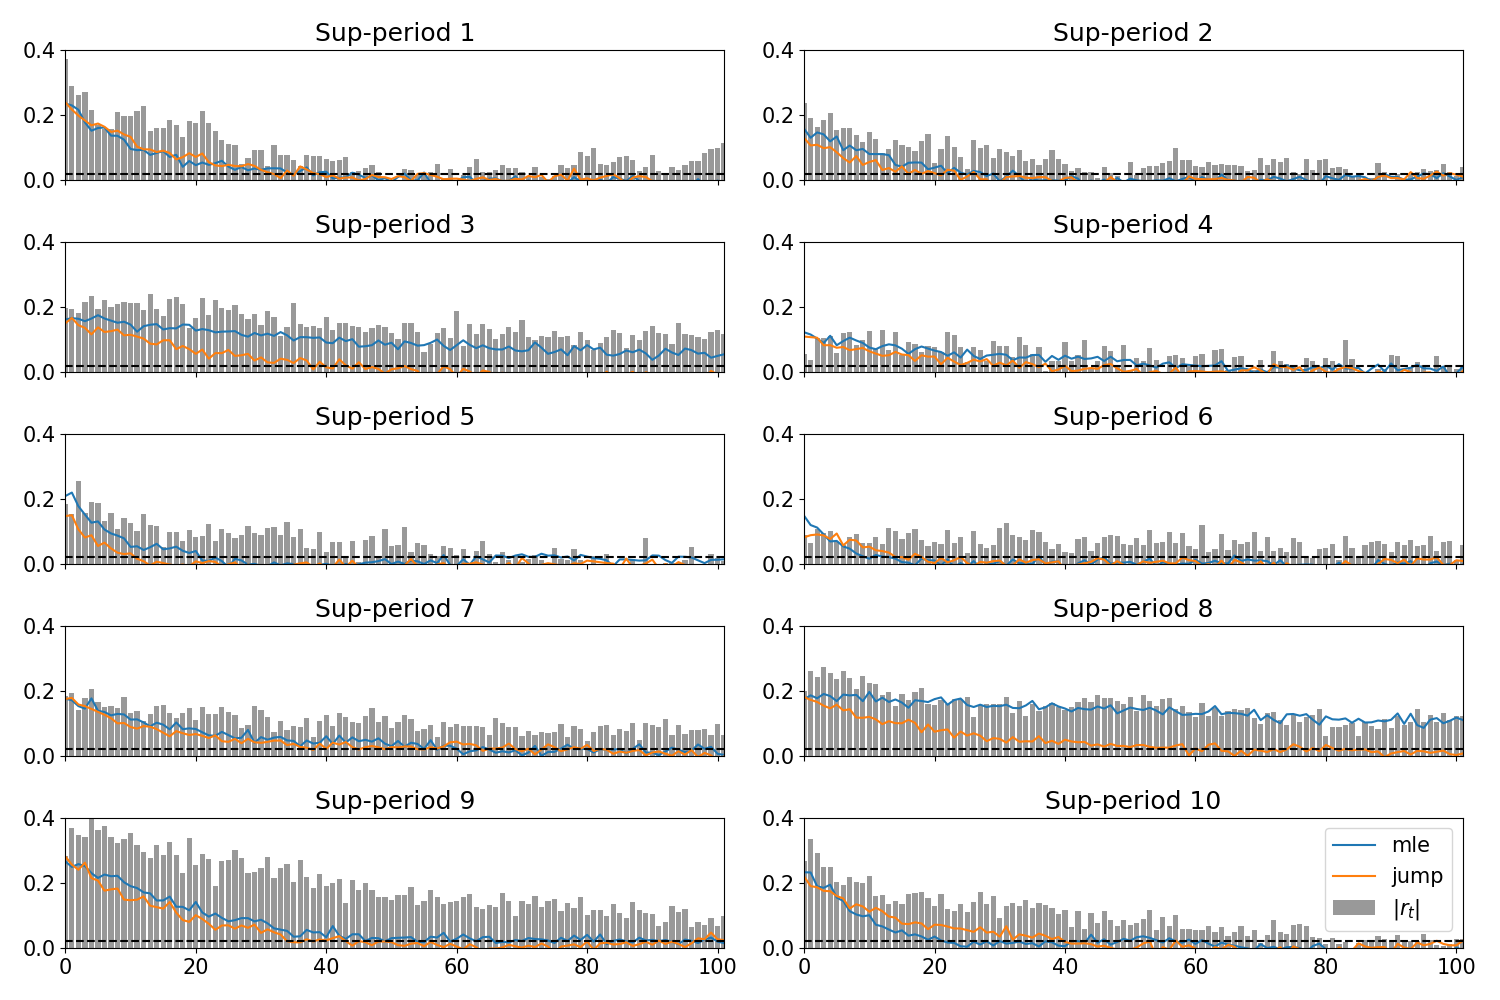
\includegraphics[width=1.0\textwidth]{analysis/stylized_facts/images/acf_abs_subperiods.png}
    \caption[Autocorrelation function of estimated models and $|r_t|$ on subsamples]{Autocorrelation function of estimated models and $|r_t|$ in a breakdown of 10 subperiods each of 1700 observations. Results are similar to those of Ryden et al. (1998) and Bulla (2011). In most periods the ACF is underestimated and both models' ACF becomes insignificant within 50 lags. \textbf{Ret stavefejl i Sub-period.}}
    \label{fig:stylized_facts_acf_plots_sub_periods} 
\end{figure}

\subsubsection{Temporal properties of the rolling model}

In order to get an overview of the full sample period, figure \ref{fig:stylized_facts_acf_plots} plots the full sample empirical absolute autocorrelation function together with the simulated absolute ACF functions of the \mle and \jump models. The black dashed line is the upper boundary of the 95\% confidence interval under the null hypothesis of independence (Madsen, 2008). The absolute autocorrelations of both the \mle and \jump model have significantly increased and is now larger than that of the data at lags above 350. Interestingly, the initial decay of both models is stronger than $|r_t|$ for the first $\sim$ 50 lags after which it flattens out.\textbf{Think about a good reason for why this might be.}
The reader should note that the persistence of the ACF of the absolute returns is, to some extent, a consequence of the aforementioned volatility clustering and the significance of the lags above lag 100 is more likely a result of the data-generating process being non-stationary as mentioned earlier. 

\begin{figure}[H] 
    \centering
    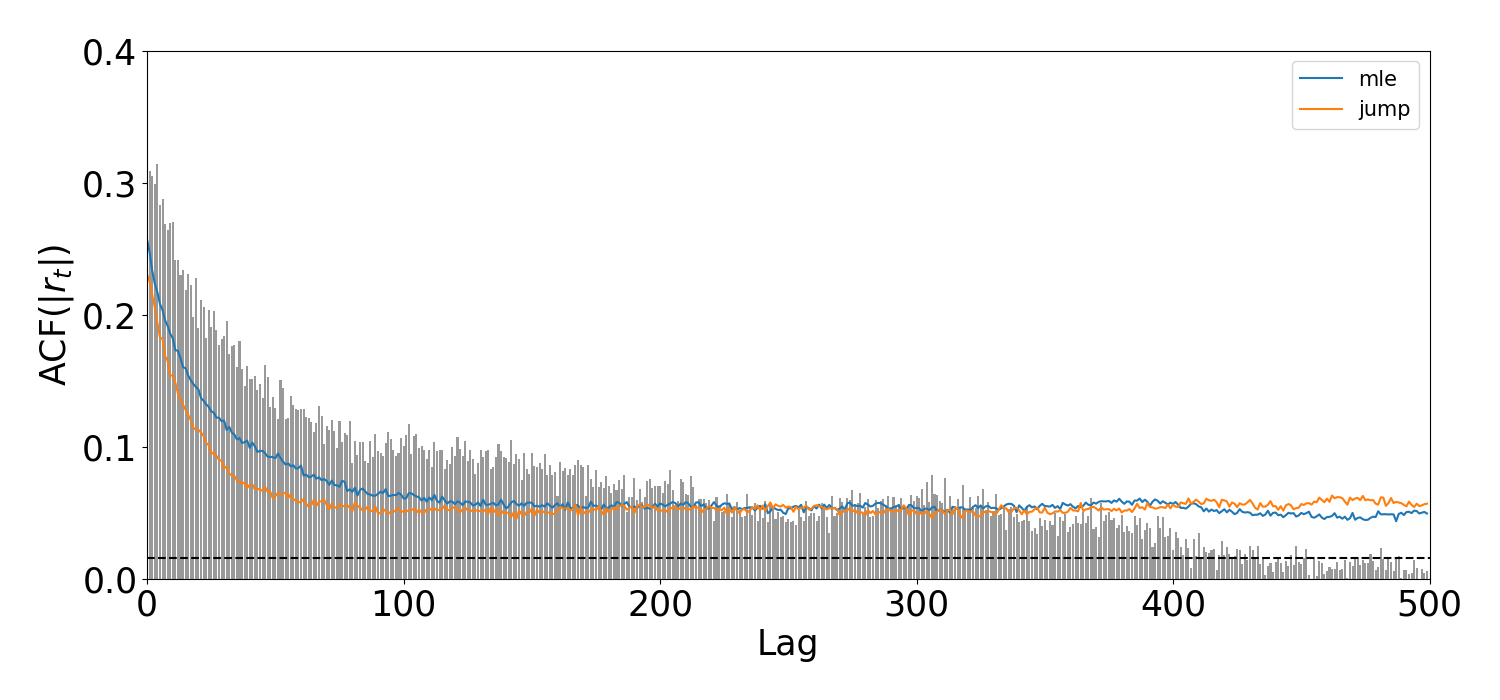
\includegraphics[width=1.0\textwidth]{analysis/stylized_facts/images/acf_abs.png}
    \caption[Autocorrelation function of estimated models as well as $|r_t|$ on full sample data]{Autocorrelation function of estimated models as well as $|r_t|$ on full sample data.}
    \label{fig:stylized_facts_acf_plots} 
\end{figure}

From the plot in figure \ref{fig:stylized_facts_acf_plots} it is also evident that the \mle model does a better job at reproducing the shape of the absolute ACF for the first 200 lags, however, the performance of the models is similar after this point. In addition, neither of the models' absolute autocorrelation become insignificant even at very large lags which is in line with the actual autocorrelation of the absolute empirical returns. The reader should note that since the computation underpinning the autocorrelation plots of figure \ref{fig:stylized_facts_acf_plots} relies on simulations, the true absolute autocorrelations are probably higher as the bouncing behaviour from the simulations exhibited in figure \ref{fig:stylized_facts_moments_bulla_abs_outliers} should reduce autocorrelation.

The remaining stylized fact is TP3, i.e. $corr(|r_t|, |r_{t-k}|) > corr(|r_t|^{\theta}, |r_{t-k}|^{\theta}) \forall \theta \neq 0$, which is often referred to as the Taylor effect. In order to analyse whether the Taylor effect holds the coefficient $\theta$ is estimated for every period by maximizing the first order autocorrelation of $|r_t|^{\theta}$. As with Rydén et al. (1998), the computation is conducted through Monte-Carlo simulations and subsequent numerical maximization. Figure \ref{fig:stylized_facts_taylor_effect} summarizes the results.

\begin{figure}[H] 
    \centering
    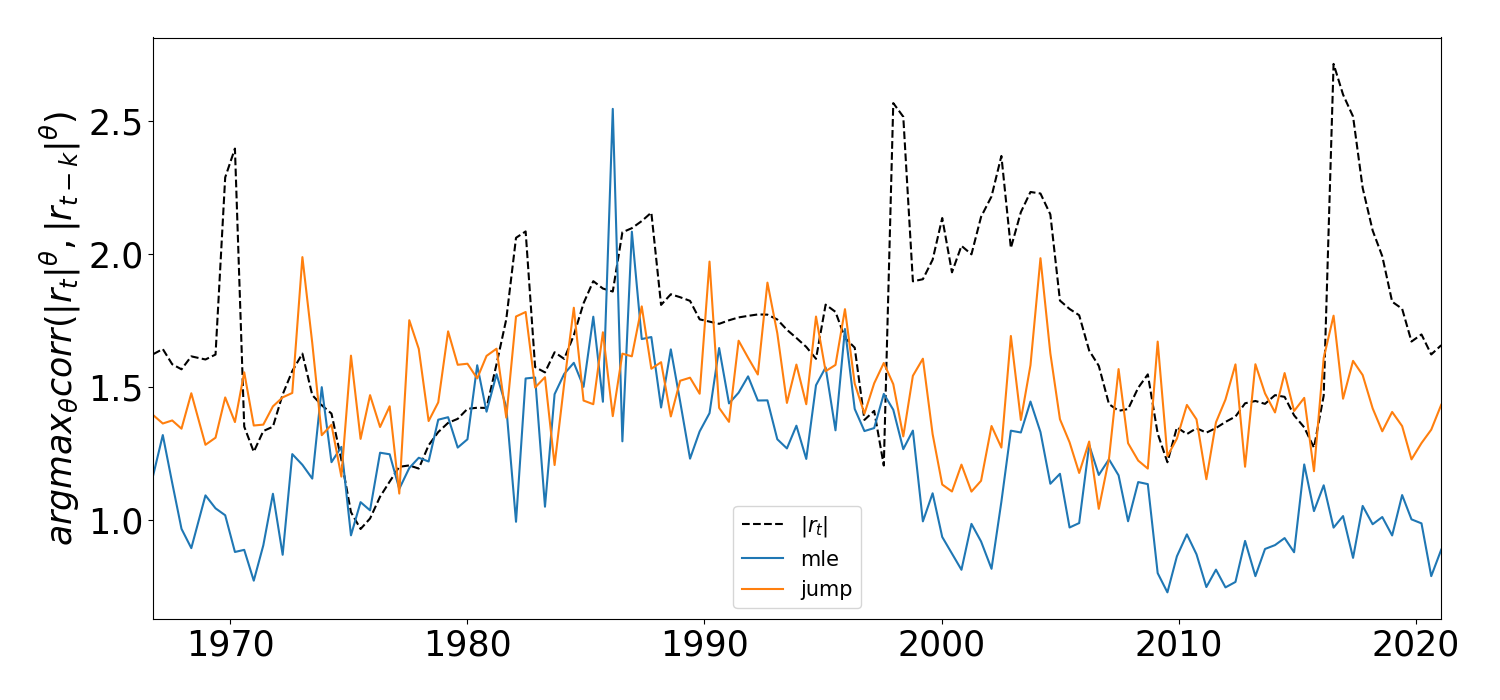
\includegraphics[width=1.0\textwidth]{analysis/stylized_facts/images/taylor_effect.png}
    \caption[Taylor effect comparison of the $\theta$ maximizing first order autocorrelations of $|r_t|^{\theta}$ and for the models]{Taylor effect comparison of the $\theta$ maximizing first order autocorrelations of $|r_t|^{\theta}$ and for the models. It is computed by Monte-Carlo simulations and subsequent use of numerical maximization.}
    \label{fig:stylized_facts_taylor_effect} 
\end{figure}

It is evident that the maximizing values of $\theta$ for the data series are not exactly equal to 1, thereby suggesting that neither models fully capture the properties stipulated by TP3. Even so, the fluctuation of both models is roughly the same as that observed by $|r_t|$, although the data fluctuates more aggressively. Apart from a smaller period from 1998 to 2005, the general direction of both models appears to follow that of the data, thereby indicating model adequacy.

\subsection{Decoding and prediction}

\textbf{This section is currently not really used for anything except showing pretty graphs as state prediction is not used in the asset allocation strategies. Should be changed to either focus on the posterior probabilities in each state, since this is used in forecasting, or something else. Otherwise delete.}

\textbf{Should be centered around 1-step density forecasts or the persistence of states in a rolling model.}

\textbf{Test if state persistence is improved on outlier-corrected data --> This can easily be done in an out-of-sample setting.}

As mentioned in section \ref{section: estimation} the hidden states are uncovered through the Viterbi algorithm. Since the estimation procedure is based on a rolling window, the state at time $t$ is estimated by using the most recent observation as well as the previous 1699. As such, the decoding procedure iterates through the entire row of observations 1 time step at a time as shown in figure \ref{fig:stylized_facts_decoded_states}. As previously mentioned, it is important to stress that the objective of this procedure is not to predict future states of the economy, but rather to identify and uncover the current state underlying the economy given past observations. 

\begin{figure}[H] 
    \centering
    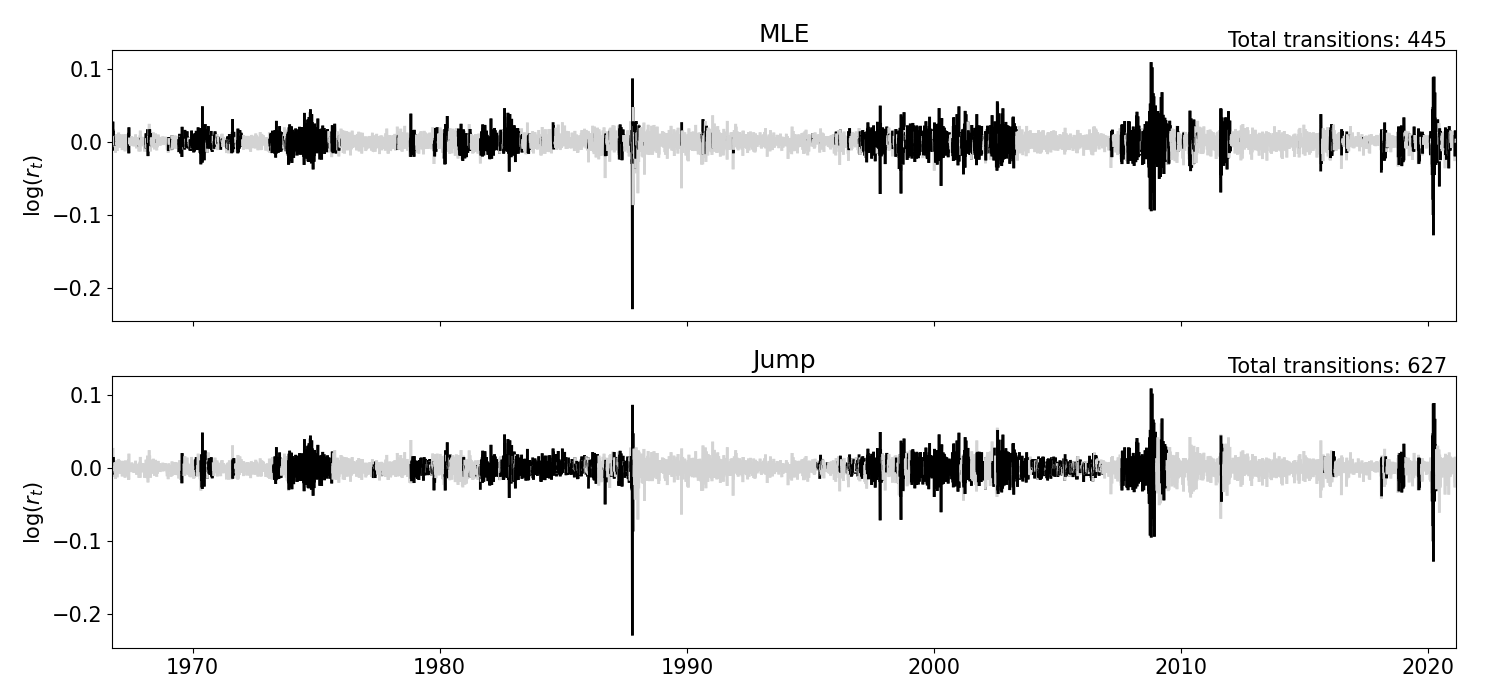
\includegraphics[width=1.0\textwidth]{analysis/stylized_facts/images/decoded_states.png}
    \caption[S\&P 500 $\log r_t$ plotted with the respective models' decoded states]{S\&P 500 $\log r_t$ plotted with the respective models' decoded states. States are decoded using a rolling window of 1700 trading days. Black indicates the high-variance state. \textbf{Fjern black monday etc. fra plot}}
    \label{fig:stylized_facts_decoded_states} 
\end{figure}

It is evident from the figure that the \mle model does a decent job in detecting the high-volatility states. However, it also appears that the model identifies some high-variance states in periods characterised by low market volatility, for instance in the beginning of the 1990s. This is most likely a result of low excess kurtosis. A similar pattern appears when analysing the decoding states of the \jump model since it too does a fairly good job at identifying the high-variance state, although the two methods disagrees in some time periods. This is for instance evident when looking at 1985 to 1990 where the \mle models suggests a low variance state, contrary to the \jump model. Furthermore, it appears that the \jump model is less consistent compared to the \mle model as it jumps around more sporadically. This is backed by the fact that the \jump model suggests 627 state transitions throughout the period which is more than 40\% more state changes compared to the suggested 445 transitions by the \mle model. This is perhaps surprisingly since the \jump framework penalizes state transitions, however, this is most likely a result of the rolling estimation approach. As such, if one were to conduct a similar analysis in which the \jump model was estimated by batches or on the full sample size, the total suggested transitions would most likely decrease, albeit these estimation procedures would introduce other problems. 

In addition, it is positive to witness that both models correctly identifies major market events such as Black monday in 1987, the dot-com bubble of the early 2000s, the GFC of 2008 and most recently the COVID-19 recession as high-variance states, albeit the models disagree in terms of how long the high-variance state persists. Furthermore, it was evident by figure \ref{fig: SP500_index} that there were short periods of large positive returns following the big market crash in September/October 2008, however, both models predict those as bear states, which indicates that variance dominates means in the prediction of whether a state is classified as high or low variance. Another aspect that has to be considered in terms of using the either model, but particularly the \jump, is the cost of changing the portfolio allocation due to a wrong signal. As evident by figure \ref{fig: SP500_index} the period from 1980 to 1990 is characterised by increasing price levels and low variance, hence the correct classification of the state should be low-variance, however, the \jump model classifies it as a high-variance state throughout the period. As such, utilising the models when forming DAA strategies should be done carefully, as the amount of transitions and possibly miss-specified states can decrease profits and Sharpe ratios substantially.  

\subsubsection{Smoothing}

\textbf{TBD. Dette afsnit har ingen værdi da vi bruger densities i forecasts - et medianfilter kan ikke implementeres i mpc approachen.}

In the previous section it became evident that the amount of transitions between the two states are high for both models with the \mle and \jump model proposing 445 and 627 transitions respectively. This amount of state transitions decreases the confidence that the uncovered state changes occur due to the economy entering a new state, while increasing the suspicion towards random sporadic jumps. Furthermore, it was evident that the \jump model proposed more than 40\% more transitions compared to the \mle, and this constitutes an issue due to the objective of \jump model being to constrain sporadic and frequent jumps. Lastly, such fluctuations and sporadic transitions can be costly in a DAA framework, especially when factoring in opportunity cost of allocating capital poorly due to a miss-specified state, and when factoring in actual trading costs. As a result of these conclusions, a probability smoothing scheme is implemented to improve persistence and hence reduce the amount of state transitions. For every state prediction at time $t$, the probability of being in all states are computed as described in section \ref{section: estimation}. This is then compared to a median threshold hence a state change will only occur if the past 4 out of 7 state predictions suggest that a change must occur. The choice of threshold is a trade-off between the time-delay in state changes and the confidence in state predictions as described by Nystrup (2014). The associated results of applying such a smoothing scheme is shown for the \mle and \jump model in figure \ref{fig:stylized_facts_decoded_states_filtered}.

\begin{figure}[H] 
    \centering
    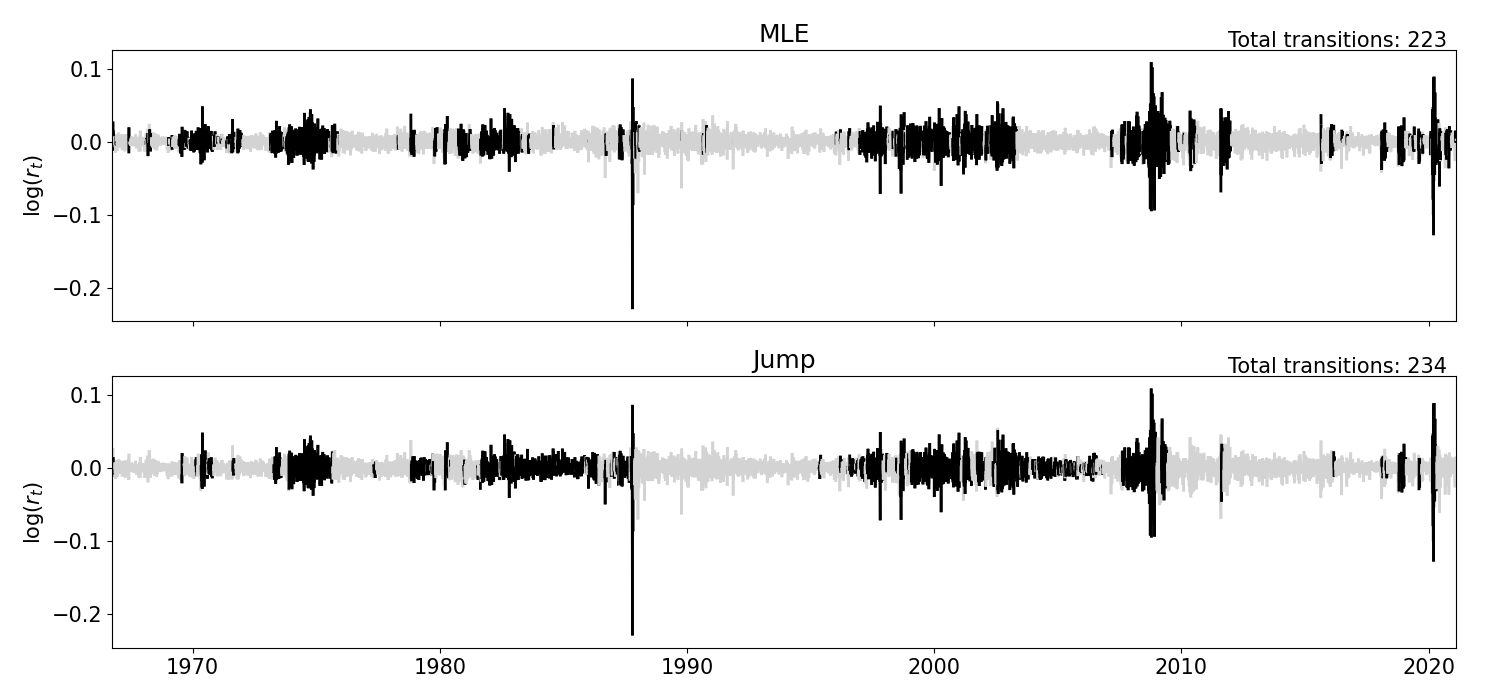
\includegraphics[width=1.0\textwidth]{analysis/stylized_facts/images/decoded_states_filter.png}
    \caption[S\&P 500 $\log r_t$ plotted with the respective models' smoothed decoded states]{S\&P 500 $\log r_t$ plotted with the respective models' smoothed decoded states. States are decoded using a rolling window of 1700 trading days.  Black indicates the high-variance state.}
    \label{fig:stylized_facts_decoded_states_filtered} 
\end{figure}

It is evident that the number of proposed transitions reduces dramatically from 445 to 223 for the \mle model and from 627 to 234 for the \jump model. The drastic decrease in transitions is primarily visible in the fewer amount of short-lived sojourn times. However, despite the apparent decrease in the number of transitions, there still appears to be inconsistency across the two models in terms of state predictions. This is once again evident in the time period from 1985 to 1990 in which the \mle model suggests low-variance states and the \jump model suggests high-variance states. Yet, both models are still able to capture the big market events as previously described. Furthermore, applying the probability smoothed models serve as a better option compared to the non-smoothed alternative in a DAA framework since the reduction in state transitions, all else equal, will reduce trading costs and increase returns. 

As conclusively remarks of section \ref{Section: Stylized facts}, it appears that both the \mle and \jump model are able to reproduce the four temporal as well as the three distributional properties, however, the \jump model does an overall better job. Particularly, when reproducing the empirical absolute autocorrelation function the \jump model achieves a better fit for the first 200 lags, although the \mle achieves a better fit for the remaining lags. Furthermore, there is a significant variation in the parameters over time, thereby greatly supporting the use of rolling estimation. In addition, the use of rolling estimation has the property that no foresight is assumed at any point in time, thereby making the prediction model likely to generalize well to new data. Lastly, a smoothing scheme has been applied when uncovering the hidden states, thereby increasing state persistence while reducing the amount of transitions between states. Despite these initiatives, it is clear that the models still provide inconsistent state predictions thereby increasing the risk of making poor capital allocation decision, and as a result encounter decreasing profits through a DAA framework. In the following sections, the MPC framework will be introduced and based on this it will be investigated whether trading strategies conditional on the predicted states are profitable.
